\begin{chapter}{\label{cha:numerics}Numerical Methods}
\section{\label{section:RK} Numerical procedures for 2D and 3D solutions}
	\subsection{\label{section:RK4} Runge-Kutta}
	\subsection{\label{section:imagTime} Imaginary time convergence}
	\subsection{\label{section:numericalParams} Numerical stability}
	We now systematically study the numerical stability of common simulated systems. Our aim is to find a suitable discretisaton of space and time so that while simulations are timely, our numerical solutions are converged and not overly sensitive to small changes computational parameters.

	We use energy to measure because in the undamped gpe energy is conserved.

	We run 100 units of imaginary time stepping to get density profile
	We run another 100 units for vortex IC
	We run 500 units in real time to study stability


\begin{figure}
	\centering
	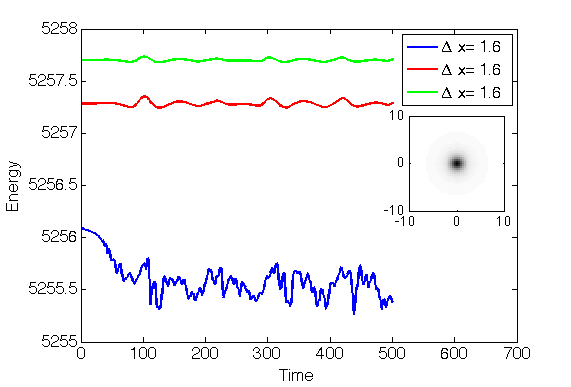
\includegraphics[width=0.5\textwidth]{numerics/figures/homg_energy_cons.png}
\end{figure}

\section{\label{section:vortexidentifying} Identifying vortices}

	\begin{algorithm}[H]
	\SetKwFunction{Zero}{Zero}
	\SetKwInOut{Input}{input}\SetKwInOut{Output}{output}
	\SetKwData{Linked}{linked}
	\SetKw{KwAnd}{and}
	\Input{A $n_x \times n_y$ field $\theta$. A $n_x \times n_y$ field $P$. A line integral width $l$.}
	\Output{A $n_x \times n_y$ field $Q$.}
	\BlankLine
	\For{$i\leftarrow 1+l/2$ \KwTo $n_x-l/2$}{
		\For{$i\leftarrow 1+l/2$ \KwTo $n_y-l/2$}{
			$Q[i,j]\leftarrow\oint_\Box \nabla\theta~ds$, where $\Box$ is a square loop of width $l$ centered on $(i,j)$\;
		}
		\lIf {$P[i,j]>1$}{$Q[i,j]\leftarrow0$}
	}


\caption{Initial vortex detection. Outputs a field with positive values near a vortex with circulation 1, negative values near a vortex with circulation -1 and zero valued otherwise.}\label{algo_calcvortexfield}
\end{algorithm}



	\begin{algorithm}[H]
	\SetKwFunction{Zero}{Zero}
	\SetKwInOut{Input}{input}\SetKwInOut{Output}{output}
	\SetKwData{Linked}{linked}
	\SetKwData{Lc}{lc}
	\SetKwData{Rc}{rc}
	\SetKwData{Call}{c}
	\SetKwData{Mtmp}{m}
	\SetKwFunction{Max}{max}
	\SetKwFunction{Min}{min}
	\SetKw{continue}{continue}
	\SetKw{KwAnd}{and}
	\Input{A $n_x \times n_y$ binary field $P$.}
	\Output{A $n_x \times n_y$ field $Q$.}
	\BlankLine
	Let \Linked be a $(n_x.n_y) \times 4$ field\;
	\Linked$\leftarrow -1$ at every point, $Q\leftarrow -1$ at every point\;
	\Lc$\leftarrow 1$, \Rc$\leftarrow 0$\;

	\For{$i\leftarrow 2$ \KwTo $n_x-1$}{
		\For{$j\leftarrow 2$ \KwTo $n_y-1$}{
			\lIf {$P[i,j] = 0$}{skip this loop iteration}
			\ForEach{\Call $\in(Q[i+1,j-1],Q[i,j-1],Q[i-1,j-1],Q[i-1,j])$}{
				\If {\Call$\geq 0$}{
					$Q[i,j]\leftarrow$\Call\;
					\Linked\!$[$\Lc$,1]\leftarrow$\Call\;
				}
			}
			\lIf{$Q[i,j] \geq 0$}{\Lc$\leftarrow$\Lc$+ 1$}
			\Else{
				Q[i,j]$\leftarrow$\Rc\;
				\Rc$\leftarrow$\Rc$+ 1$\;
			}
		}
	}
	\For{$i\leftarrow 1$ \KwTo $(n_x \times n_y)$}{
		\lIf{\Max{All elements of \Linked from row $i$}$= -1$}{\continue}
		\Mtmp $\leftarrow$ \Min{All elements of \Linked from row $i$ with value$\geq 0$}\;

		\For{$j\leftarrow 1$ \KwTo $4$}{
			\If{\Linked\!$[i,j] \neq\,$\Mtmp \KwAnd \Linked\!$[i,j] \geq 0$ }{
				\For{$k\leftarrow 1$ \KwTo $n_x$}{
					\For{$l\leftarrow 1$ \KwTo $n_y$}{
						\lIf{$Q[k,l]  =$~\Linked\!$[i,j]$}{$Q[k,l] = $~\Mtmp}
					}
				}
			}
		}
	}


\caption{The B/W Label algorithm. Outputs a field with the same non-zero regions of the input binary field, but with each connected region labeled with a unique value.}\label{algo_bwlabel}
\end{algorithm}


	\subsection{\label{section:gaussianblur} Image filters and the Gaussian kernel}
		\begin{algorithm}[H]
		\SetKwInOut{Input}{input}\SetKwInOut{Output}{output}
		\Input{A $n_x \times n_y$ field $P$, a Gaussian filter width $g$.}
		\Output{A $n_x \times n_y$ field $Q$.}
		\BlankLine
		$Q\leftarrow0$ at every point\;
		\For{$k\leftarrow 1$ \KwTo $n_x$}{
			\For{$l\leftarrow 1$ \KwTo $n_y$}{
				\For{$i\leftarrow 1$ \KwTo $n_x$}{
					\For{$j\leftarrow 1$ \KwTo $n_y$}{
						$Q[k,l] \leftarrow Q[k,l] + P[i,j]\times\exp\left (-[(k-i)^2+(l-j)^2]/g^2 \right )$\;
					}
				}
				$Q[k,l] \leftarrow Q[k,l]/(n_x \times n_y)$\;
			}
		}

	\caption{Gaussian convolution. Filters out features with structures of size less than the input
	filter width. The output is analagous to a `blurring' of the input field. This allows high frequency noise to be removed.}\label{algo_gaussconv}
	\end{algorithm}


	\begin{algorithm}[H]
	\SetKwFunction{Zero}{Zero}
	\SetKwInOut{Input}{input}\SetKwInOut{Output}{output}
	\SetKwData{Linked}{linked}
	\SetKw{KwAnd}{and}
	\SetKwFunction{Max}{max}
	\SetKwFunction{Min}{min}
	\SetKwData{Call}{C}
	\Input{A $n_x \times n_y$ field $\theta$. A $n_x \times n_y$ field $P$. A threshold value $t$.}
	\Output{Number of vortices found, $n_v$. Vortex location, a $2 \times n_v $ field $V_l$. Vortex polarity, a vector $V_p$ of length $n_v$.}
	\BlankLine
	$Q\leftarrow$ Algorithm \ref{algo_gaussconv} $\leftarrow$ Algorithm \ref{algo_calcvortexfield} $\leftarrow(\theta,P)$ \;
	$R\leftarrow0$ at every point, $S\leftarrow0$ at every point\;
	$n_v\leftarrow 0$\;
	\For{$i\leftarrow 1$ \KwTo $n_x$}{
		\For{$j\leftarrow 1$ \KwTo $n_y$}{
			\lIf {$Q[i,j]>t$}{$R[i,j] = 1$}
			\lIf {$Q[i,j]<t$}{$S[i,j] = 1$}
		}
	}

	\ForEach{$C\in(R,S)$}{
		$D\leftarrow$ Algorithm \ref{algo_bwlabel} $\leftarrow C$\;
		\For{$i\leftarrow 1$ \KwTo \Max($D$)}{
			$V[1,n_v]\leftarrow$ mean row of the points where $D=i$\;
			$V[2,n_v]\leftarrow$ mean column of the points where $D=i$\;
			\lIf {$C=R$}{$V[3,n_v]\leftarrow 1$}
			\lIf {$C=S$}{$V[3,n_v]\leftarrow -1$}
			$n_v \leftarrow n_v + 1$\;
		}
	}

	\caption{Calculate vortex locations and polarity.}\label{algo_calcvortexlocs}
	\end{algorithm}



\section{\label{section:vortexclustering} Quantifying vortex clustering}
	\subsection{\label{section:reevesalgorithm} Recursive Cluster Algorithm (RCA) }
		\begin{algorithm}[H]
		\SetKwFunction{Zero}{Zero}
		\SetKwInOut{Input}{input}\SetKwInOut{Output}{output}
		\SetKwData{Linked}{linked}
		\SetKw{KwAnd}{and}
		\SetKwFunction{Max}{max}
		\SetKwFunction{Min}{min}
		\SetKw{continue}{continue}
		\SetKw{or}{or}
		\SetKw{and}{and}
		\SetKwData{Call}{C}
		\Input{Vortex location, a $2 \times n_v $ field $V_l$. Vortex polarity, a vector $V_p$ of length $n_v$. Number of vortices, $n_v$.}
		\Output{Vortex decomposition, a vector $V_{\mathrm{rca}}$ of length $n_v$.}
		\BlankLine
		$n_{\mathrm{rca}}\leftarrow0$\;
		$V_{\mathrm{rca}}\leftarrow 0$ at every point\;
		\While{dipoles continue to be identified}{
			\For{$i\leftarrow 1$ \KwTo $n_v$}{
				\If {vortex $i$ is mutual nearest neighbours with some other vortex $j$}{
				\If {$V_p[i] \neq V_p[i]$}{
						$V_{\mathrm{rca}}[i] \leftarrow -1$\;
						$V_{\mathrm{rca}}[j] \leftarrow -1$\;
					}
				}
			}
		}
		\While{vortices continue to be added to clusters}{
			\For{$i\leftarrow 1$ \KwTo $n_v$}{
				\For{$j\leftarrow 1$ \KwTo $n_v$}{
					\lIf {$V_{\mathrm{rca}}[i] < 0$ \or $V_{\mathrm{rca}}[j]<0$}{\continue}
					\If {vortex $i$ and $j$ are closer to one another than one of opposite polarity}{
						\lIf {$V_{\mathrm{rca}}[i] > 0$ \and $V_{\mathrm{rca}}[j] = 0$}{$V_{\mathrm{rca}}[j]\leftarrow V_{\mathrm{rca}}[i]$}
						\lElseIf {$V_{\mathrm{rca}}[i] = 0$ \and $V_{\mathrm{rca}}[j] > 0$}{$V_{\mathrm{rca}}[i]\leftarrow V_{\mathrm{rca}}[j]$}
						\lElseIf {$V_{\mathrm{rca}}[i] > 0$ \and $V_{\mathrm{rca}}[j] > 0$}{($V_{\mathrm{rca}}=V_{\mathrm{rca}}[i]) \leftarrow V_{\mathrm{rca}}[j]$}
						\Else{
							$n_{\mathrm{rca}} \leftarrow n_{\mathrm{rca}} + 1$\;
							$V_{\mathrm{rca}}[i]\leftarrow n_{\mathrm{rca}}$\;
							$V_{\mathrm{rca}}[j]\leftarrow n_{\mathrm{rca}}$\;
							}
					}
				}
			}
		}

		\caption{The Recursive Cluster Algorithm. Decomposes a list of vortices into vortex dipoles or clusters. Vortices are labelled with a cluster number, with vortex diploes labeled with $-1$.}\label{algo_vortexkiller}
		\end{algorithm}


	\subsection{\label{section:ripleysk} Ripley's K function }
		\begin{equation}\label{eq:ripleysk}
		K(x) = \frac{A}{n^2}\sum\limits_{i \ne j} I\left (d_{ij}<x\right ),
		\end{equation}
		where $d_{ij}$ is the distance between the $i$th and $j$th points, $A$ is the area of the region containing every point, $n$ is the number of points, $x$ is the search radius, and I is the indicator function (1 if its argument is true, 0 otherwise). Should the points be distributed homogeneously in space, then $K(s)\approx\pi s^2$.
\section{\label{section:vortextracking} Tracking vortex trajectories}
\section{\label{section:vortexremoval} Removing vortices with phase unwrapping}
	\begin{algorithm}[H]
	\SetKwFunction{Zero}{Zero}
	\SetKwInOut{Input}{input}\SetKwInOut{Output}{output}
	\SetKwData{Linked}{linked}
	\SetKw{KwAnd}{and}
	\SetKwFunction{Max}{max}
	\SetKwFunction{Min}{min}
	\SetKwFunction{Phase}{phase}
	\SetKwData{Call}{C}
	\Input{A $n_x \times n_y$ complex field $\psi$. A `safe' distance $d$. Vortex core radius $c$. }
	\Output{A $n_x \times n_y$ complex field $\phi$.}
	\BlankLine
	$\phi \leftarrow \psi$\;
	$(n_v,V_l,V_p)\leftarrow$ Algorithm \ref{algo_calcvortexlocs}~$\leftarrow\psi$\;

	\For{$i\leftarrow 1$ \KwTo $n_v$}{
		\If{$|V_l[i]| > d$}{
			Imprint a vortex of polarity $V_p[i]$ at location $V_l[i]$ in $\phi$\;
			\For{$j\leftarrow -c$ \KwTo $c$}{
				\For{$k\leftarrow -c$ \KwTo $c$}{
						$x \leftarrow V_l[1,i]+j$\;
						$y \leftarrow V_l[2,i]+k$\;
						\mbox{$\phi(x,y) \leftarrow \psi_{\inf}~\times$~\Phase{$\psi(x,y)$}\;}
				}
			}
		}
	}

	\caption{The `vortex killer' algorithm. By accurately imprinting a vortex, this algorithm removes vortices from the input wavefunction non destructively.}\label{algo_vortexkiller}
	\end{algorithm}

\end{chapter}
